\documentclass[12pt]{article}
\usepackage[a4paper,left=1.5cm,right=1.5cm,top=1.5cm,bottom=1.5cm]{geometry}
\usepackage{graphicx}	
\begin{document}
	
	\begin{figure}[h!]
		
\includegraphics[scale=1]{ufpbde}
	\end{figure}
\par \textbf{Nome:} \underline{Paulo Ricardo Seganfredo Campana} \hspace{+12pt} \textbf{Matricula:} \underline{20210044220} \hspace{+12pt} \textbf{Nota:} 

	\begin{figure}[h!]
		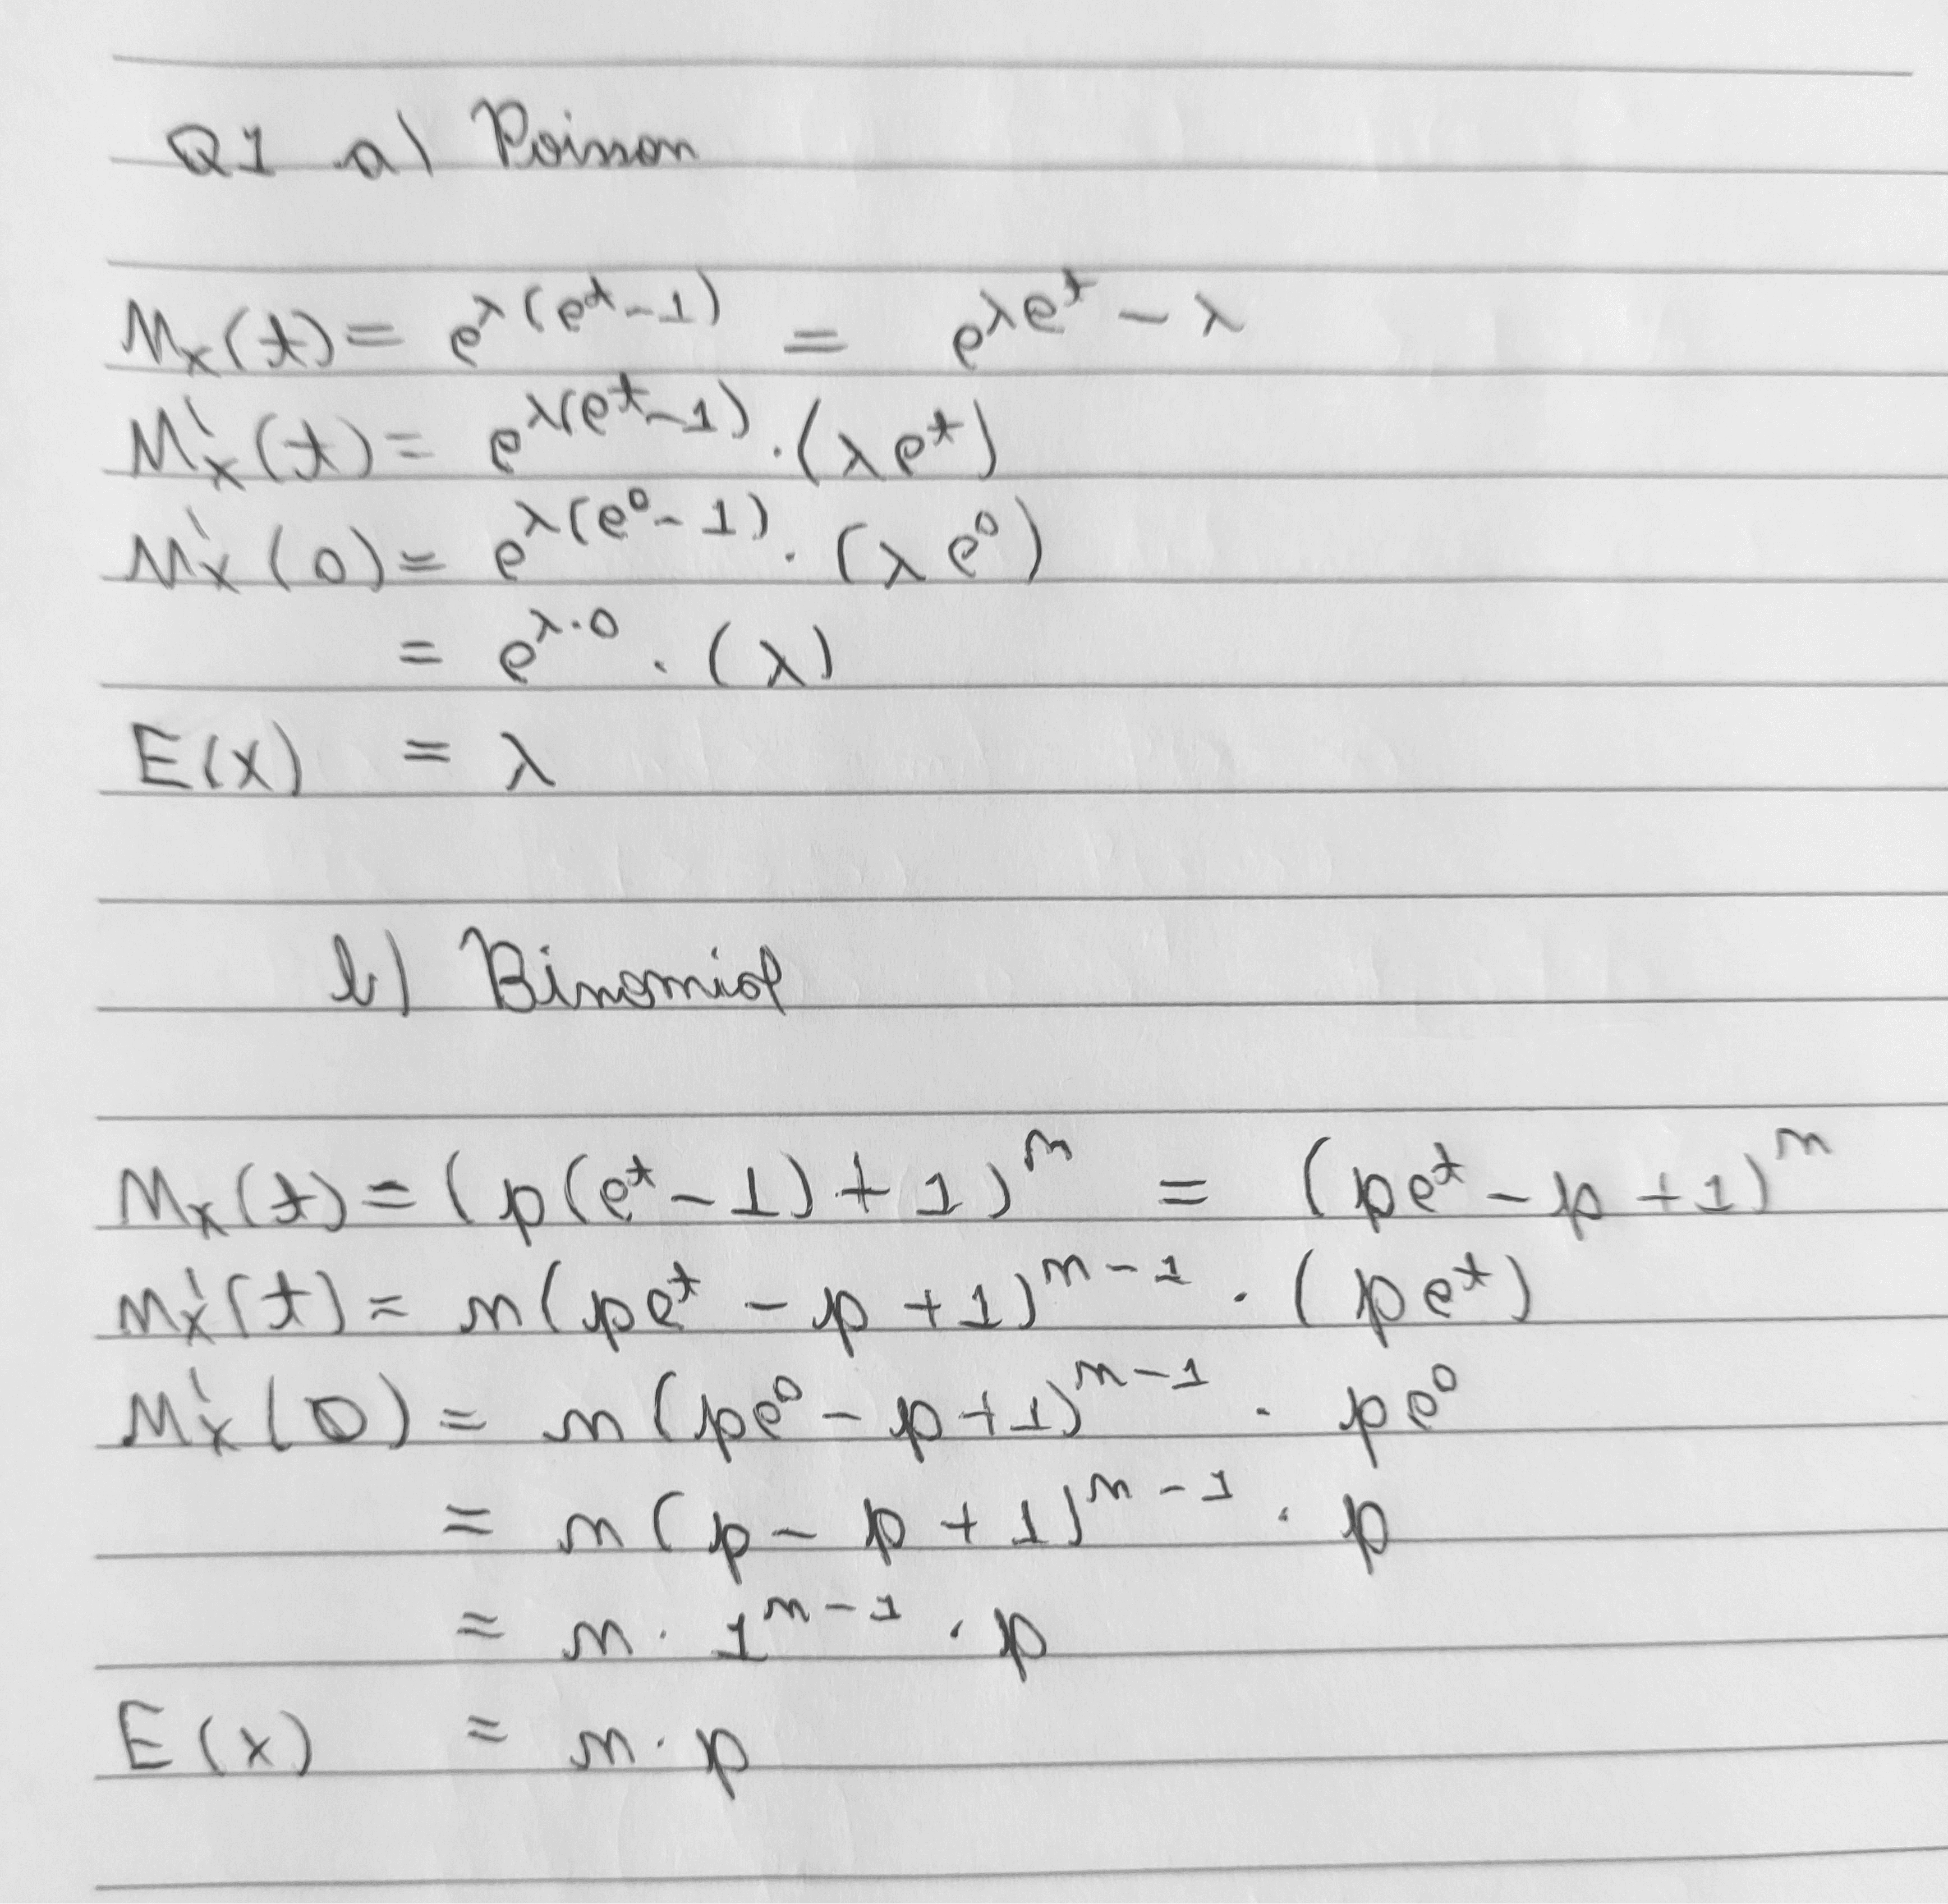
\includegraphics[scale=0.2]{q1}
	\end{figure}

	\begin{figure}[h!]
		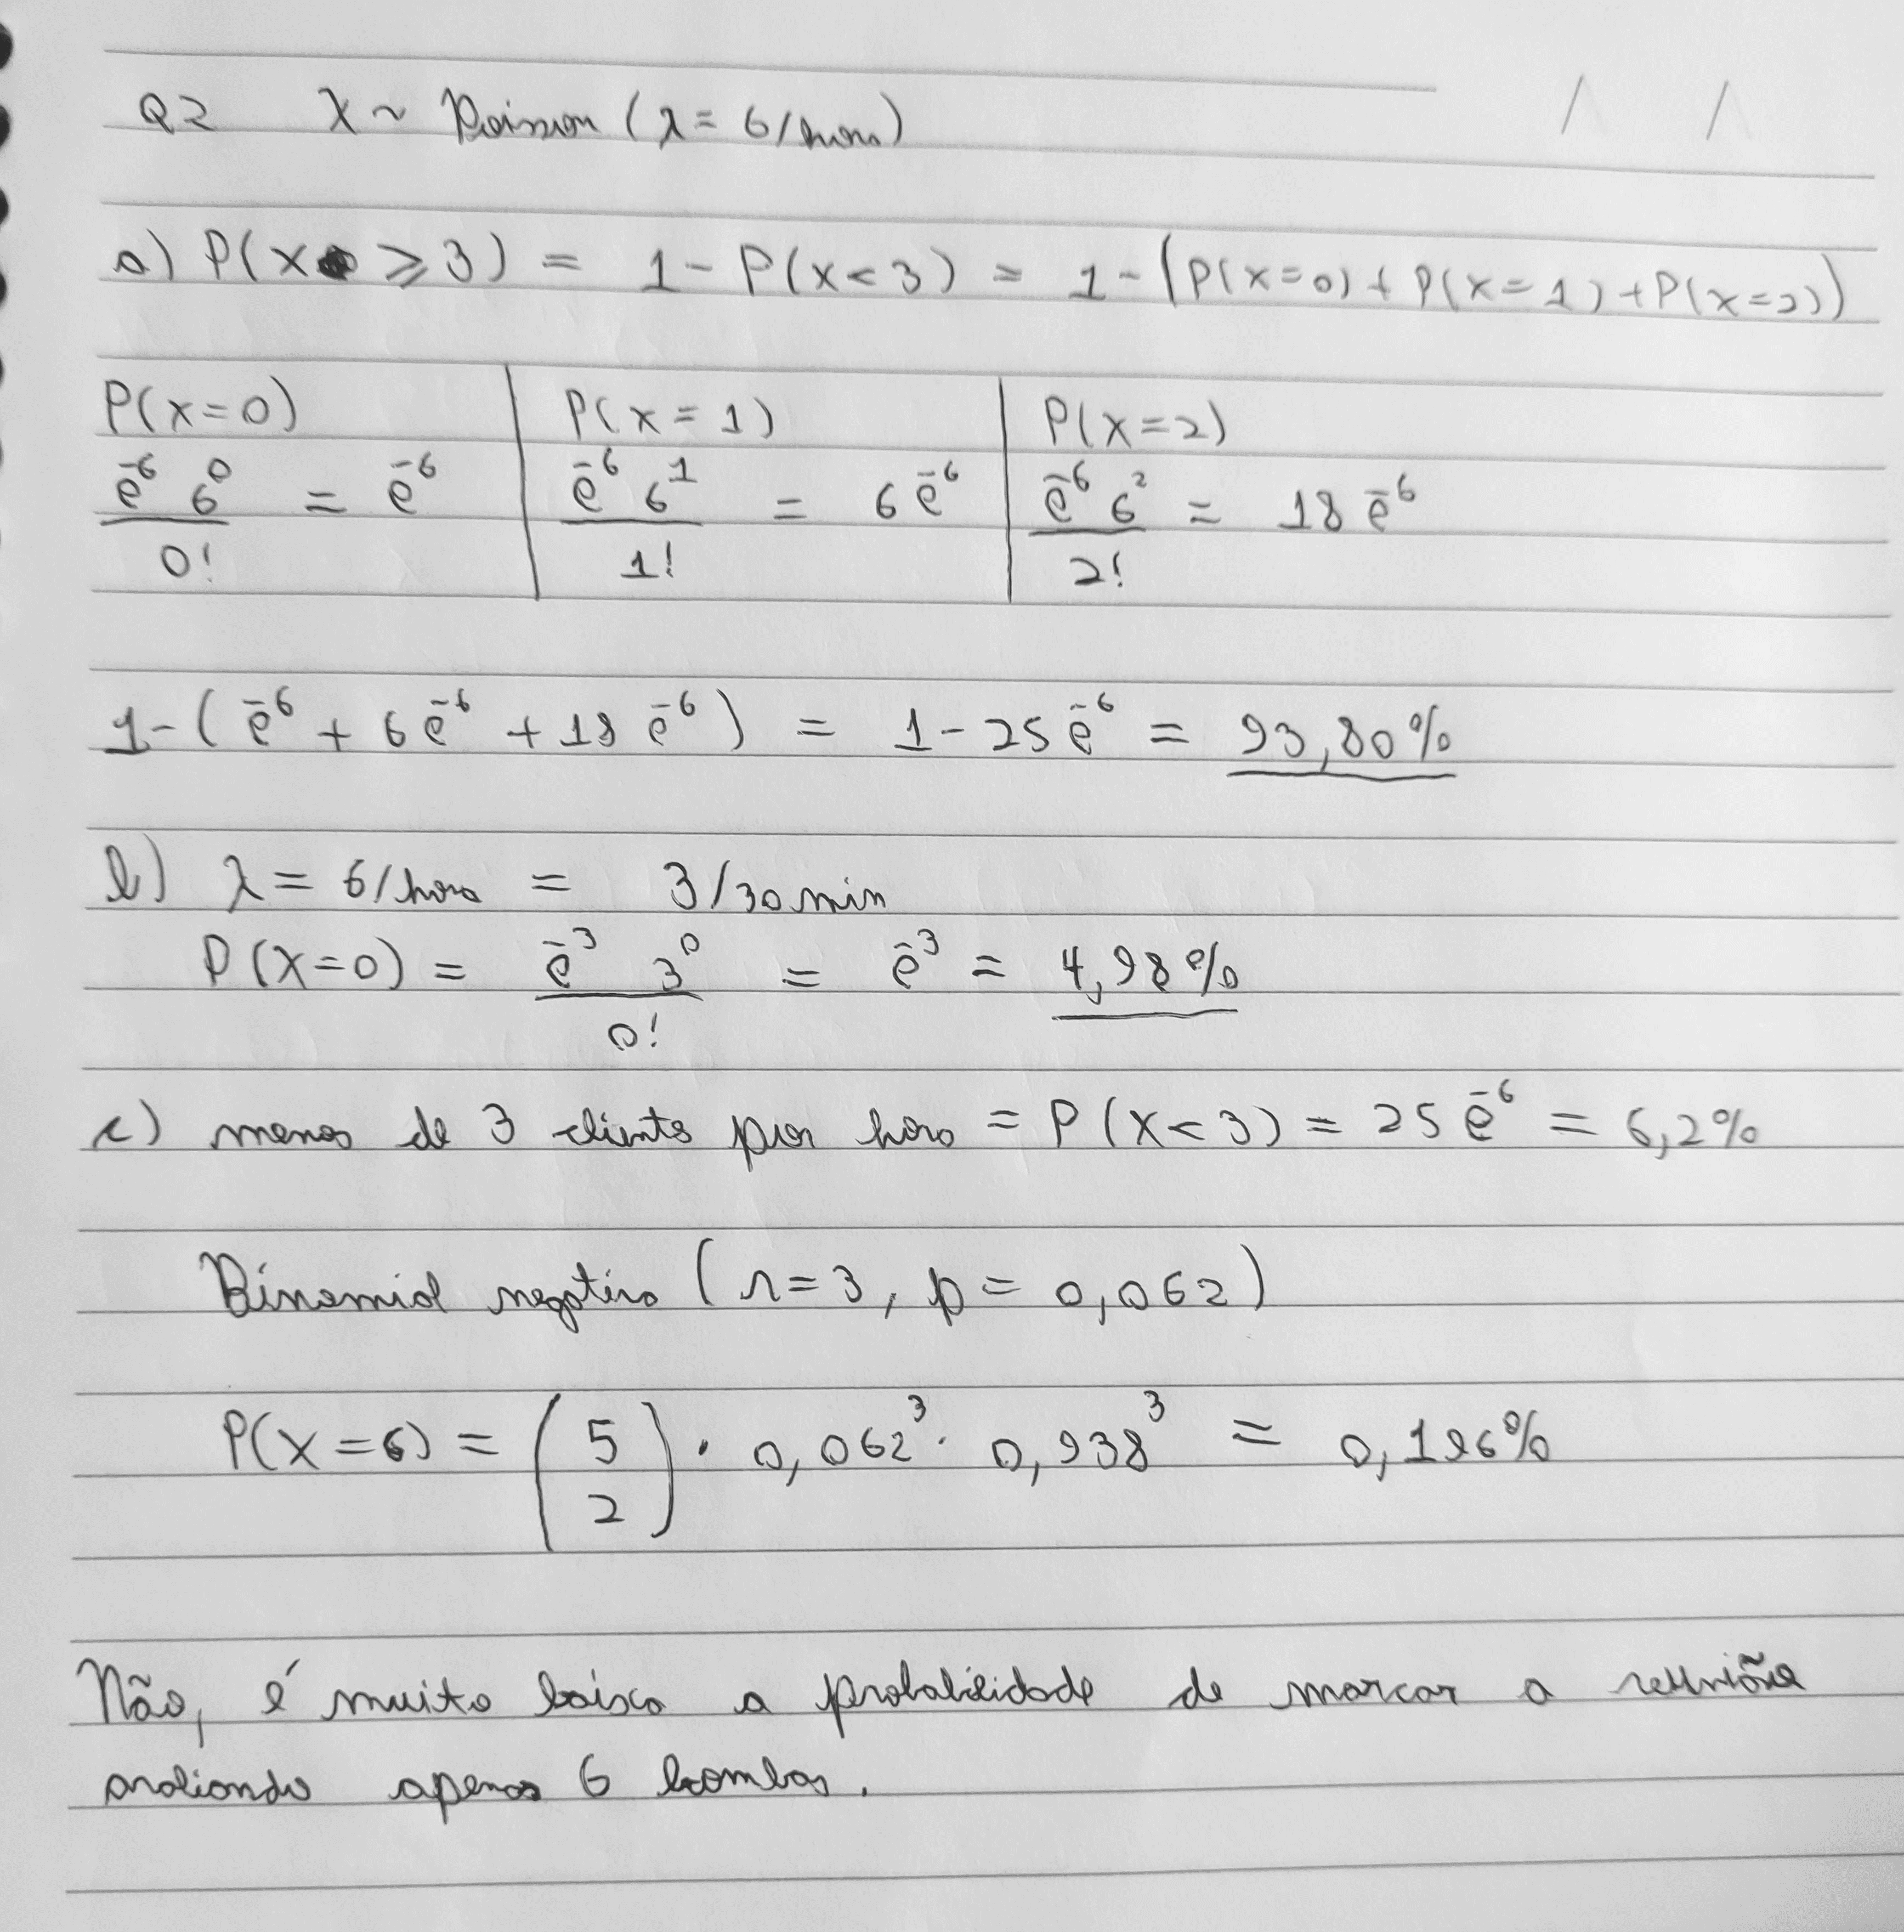
\includegraphics[scale=0.2]{q2}
	\end{figure}

	\begin{figure}[h!]
		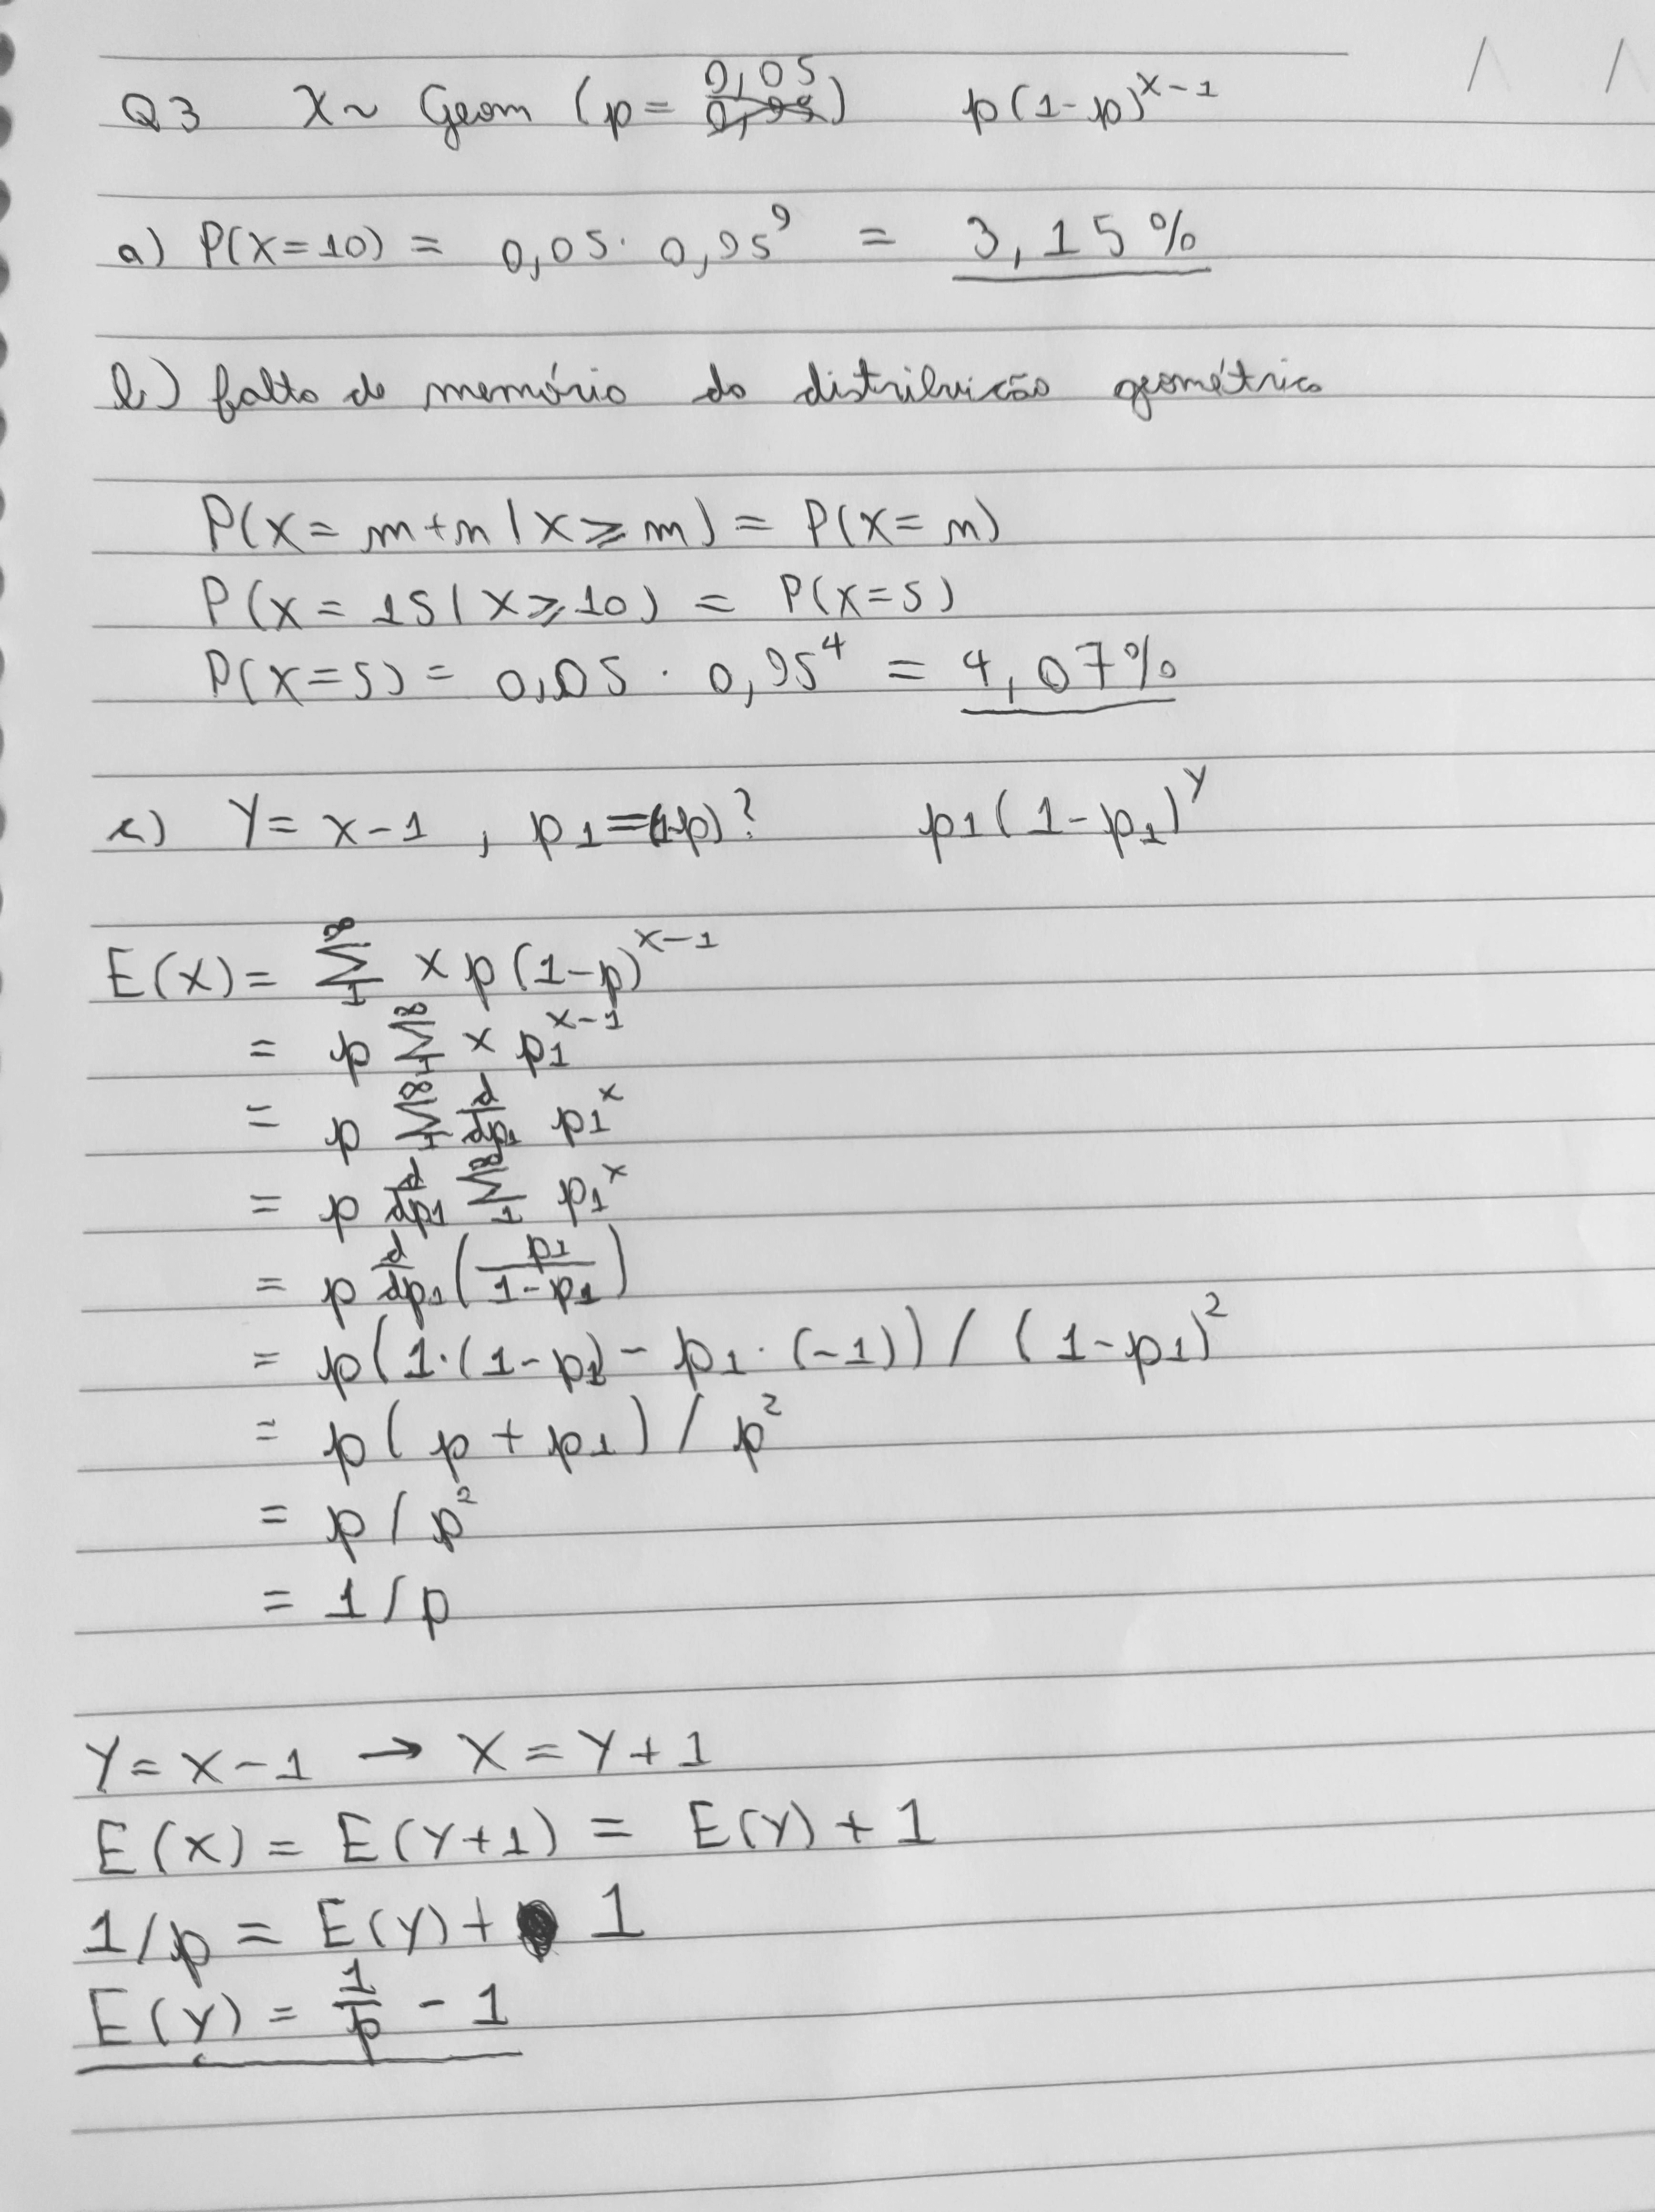
\includegraphics[scale=0.2]{q3}
	\end{figure}

	\begin{figure}[h!]
		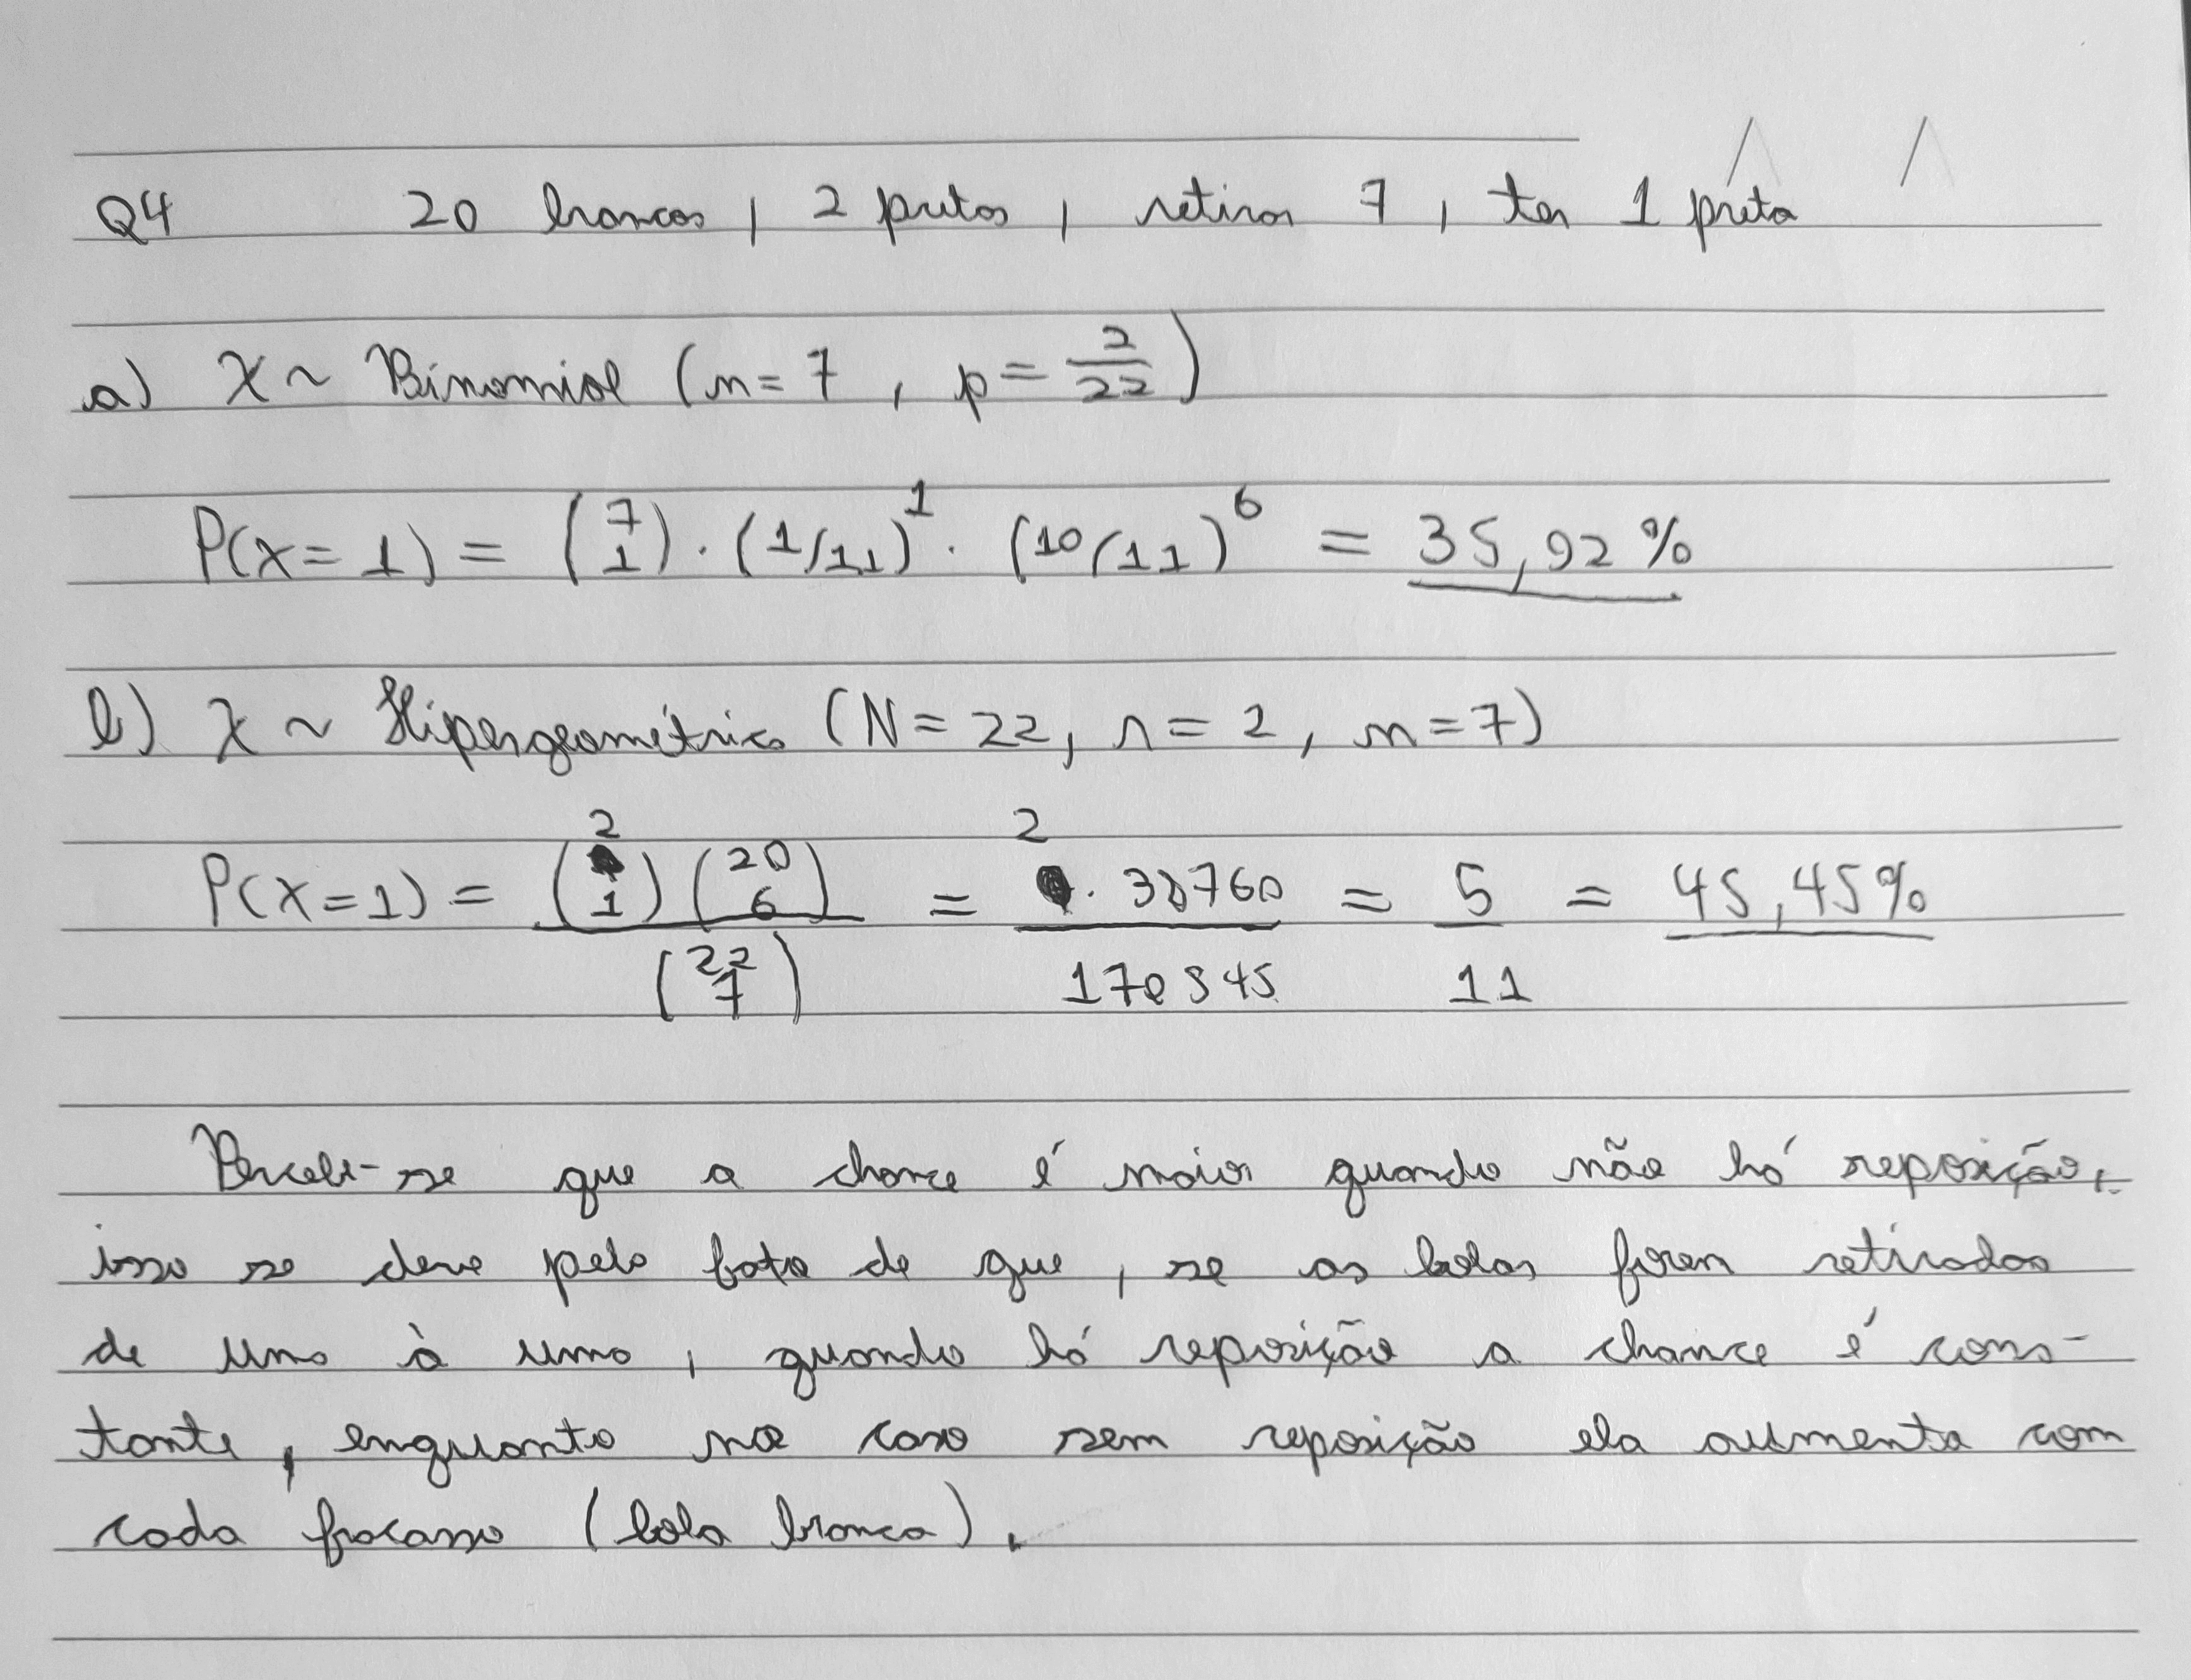
\includegraphics[scale=0.2]{q4}
	\end{figure}

\end{document}